\chapter{Hardware Implementation} \label{chap:hardware}
This chapter describes the process of implementing the system built in previous chapters on the physical robot. 
% \ac{ros} is used 
% for the hardware implementation, first the \ac{ros} data types are defined, after which the control and analysis system running on the base station
% is described. Next the systems running on board the robot are described.

\section{ROS Nodes}
There are various ros nodes spread out across the base station, the Jetson Nano and the Teensy \ac{mcu}, figure \ref{fig:nodes} provides and overview
of the nodes and how they communicate with each other. Section \ref{sec:base_ros} and \ref{sec:on_board_ros} go into detail on the publishers and subscribers
on board the robot and on the base station.

\newpage
\section{ROS Base Station} \label{sec:base_ros}
    The base station wirelessly communicates with the robot to send commands and receive data.
    For a description of the base station publishers see table \ref{tab:base_pubs} and for its subscribers see \ref{tab:base_subs}. Table \ref{tab:data_types} describes
    data types used.
    \begin{table}[h]
        \centering
        \begin{tabularx}{\textwidth}{| l | l | X | l |}
            \hline
            \multicolumn{4}{|c|}{\textbf{Base Station Publishers}} \\ \hline
            \textbf{Name} & \textbf{Data Type} & \textbf{Description} & \textbf{Frequency} \\ \hline
            % walk\_dir & Description & Data Type & Frequency \\ \hline
            command\_data & HexapodCommands & Various robot command parameters. & On change \\ \hline
            mode & Int32 & Specifies the oporationg mode of the robot. & On change. \\ \hline
        \end{tabularx}
        \caption{Base station publishers}
        \label{tab:base_pubs}
    \end{table}
    
    \noindent
    The robot currently only has two operating modes, torque cutoff mode and walking mode. The torque cutoff mode is the initial mode the robot is in,
    while in this mode the leg servos disable all torque control, thus entering a relaxed state. In walking mode the robot walks in the commanded direction
    whilst optimising its foot positions according to the terrain. If the robot encounters a piece of terrain for which no optimisation can be found the
    human controller will have to adjust the walking direction from the base station.

    \begin{table}[h]
        \centering
        \begin{tabularx}{\textwidth}{| l | l | X |}
            \hline
            \multicolumn{3}{|c|}{\textbf{Base Station Subscribers}} \\ \hline
            \textbf{Name} & \textbf{Data Type} & \textbf{Description} \\ \hline
            % walk\_dir & Description & Data Type & Frequency \\ \hline
            rgb\_data & Image & The processed color image from the robot. \\ \hline
            d\_data & Image & The processed color depth from the robot. \\ \hline
            hmap\_data & Image & The heightmap generated on the robot. \\ \hline
            LOGDATA & String & General logs from the robot. \\ \hline
        \end{tabularx}
        \caption{Base station subscribers}
        \label{tab:base_subs}
    \end{table}
    
    \noindent
    The only subscribers present on the base station are the processed camera images, heightmap and logs. These are all used to provide a interface from where
    the operator can control the robot.

\section{ROS On Board} \label{sec:on_board_ros}
    The hexapod has two computational units on board, first the Jetson Nano, which handles all high level operations, including heightmap generation and scoring,
    foot optimisation, maintain a walking gait and localisation using ORB-SLAM3. Secondly a Teensy2.0 \ac{mcu} handles low level operations, including interpolating feet movement paths
    and servo control. Table \ref{tab:jetson_pubs} to \ref{tab:teensy_subs} describe the \ac{ros} publishers and subscribers present on these two computational units.
    \begin{table}[h]
        \centering
        \begin{tabularx}{\textwidth}{| l | l | X | l |}
            \hline
            \multicolumn{4}{|c|}{\textbf{Jetson Publishers}} \\ \hline
            \textbf{Name} & \textbf{Data Type} & \textbf{Description} & \textbf{Frequency} \\ \hline
            % walk\_dir & Description & Data Type & Frequency \\ \hline
            effector\_targets & EffectorTargets & Data indicating which feet to move where, and what type of interpolation to use. & On change\\ \hline
            rgb\_data & Image & The processed color image from the \ac{rgbd} camera. & 15Hz. \\ \hline
            d\_data & Image & The processed depth image from the \ac{rgbd} camera. & 15Hz. \\ \hline
            hmap\_data & Image & The heightmap generated on the robot. & 15Hz. \\ \hline
            position & Vector3 & The localised position of the robot & 15Hz \\ \hline
            rotation & Quat & The localised rotation of the robot & 15Hz \\ \hline
        \end{tabularx}
        \caption{Jetson publishers}
        \label{tab:jetson_pubs}
    \end{table}

    \noindent
    The camera data, heightmap data, position and rotation are published for display at the base station.
    While the effector targets are published for use on the Teensy to move the robot's feet to the optimised positions.
    \begin{table}[h]
        \centering
        \begin{tabularx}{\textwidth}{| l | l | X |}
            \hline
            \multicolumn{3}{|c|}{\textbf{Jetson Subscribers}} \\ \hline
            \textbf{Name}  & \textbf{Data Type} & \textbf{Description} \\ \hline
            % walk\_dir & Description & Data Type & Frequency \\ \hline
            command\_data & HexapodCommands & Commands from the base station. \\ \hline
            color/image\_raw & Image & Raw color image from the \ac{rgbd} camera. \\ \hline
            aligned\_depth\_to\_color/image\_raw & Image & Raw depth image from the \ac{rgbd} camera. \\ \hline
        \end{tabularx}
        \caption{Jetson subscribers}
        \label{tab:jetson_subs}
    \end{table}

    As can be seen from table \ref{tab:jetson_subs} the only subscribers required on the Jetson is the raw camera feed, 
    for constructing the heightmap, and the commands from the base station.

    Table \ref{tab:teensy_pubs} show that the Teensy publishes the current feet positions these are the positions calculated through \ac{fk}. Additionally
    log data is also published for use on the base station.
    \begin{table}[h]
        \begin{tabularx}{\textwidth}{| l | l | X | l |}
            \hline
            \multicolumn{4}{|c|}{\textbf{Teensy Publishers}} \\ \hline
            \textbf{Name} & \textbf{Data Type} & \textbf{Description} & \textbf{Frequency} \\ \hline
            LOGDATA & String & General logs. & 10Hz \\ \hline
            effector\_current\_position & Eigen::Vector3d & Current feet positions. & 10Hz \\ \hline
        \end{tabularx}
        \caption{Teensy publishers}
        \label{tab:teensy_pubs}
    \end{table}
    \begin{table}[h]
        \centering
        \begin{tabularx}{\textwidth}{| l | l | X |}
            \hline
            \multicolumn{3}{|c|}{\textbf{Jetson Subscribers}} \\ \hline
            \textbf{Name} & \textbf{Data Type} & \textbf{Description} \\ \hline
            % walk\_dir & Description & Data Type & Frequency \\ \hline
            command\_data & HexapodCommands & The color image from the \ac{rgbd} camera. \\ \hline
            effector\_targets & EffectorTargets & Data indicating which feet to move where, and what type of interpolation to use.\\ \hline
            mode & Int32 & Receives mode data from the base station \\ \hline
        \end{tabularx}
        \caption{Teensy subscribers}
        \label{tab:teensy_subs}
    \end{table}

    \noindent
    Lastly, from table \ref{tab:teensy_subs} it can be seen that the Teensy subscribes to the command data, effector targets and mode.
    The walking speed component from the command data is used to set the rotational rate of the servos, as discussed in section \ref{sec:ang_rate}.
    The effector targets are used to interpolate a curve for the feet to move along, as described in section \ref{sec:arc_generation}. The mode is required
    as some modes could integrate directly with the servo control, namely the torque cutoff mode.

\newpage
\section{ROS Data Types}
    Various custom \ac{ros} data types are defined to assist with communication, these data types are described in table \ref{tab:data_types}.
    \begin{table}[h]
        \centering
        \begin{tabularx}{\textwidth}{| l | p{\widthof{float32\([2]\) walk\_dir}} | X |}
            \hline
            \textbf{Name} & \textbf{Type Definition} & \textbf{Description} \\ \hline
            % walk\_dir & Description & Data Type & Frequency \\ \hline
            Vector3 & float\([3]\) data. & A vector in 3D space.  \\
            \hline
            EffectorTargets & Vector3\([6]\) targets \newline 
                            bool\([6]\) swinging. & Data describing the targets of the robot's feet and which feet are swinging. \\
            \hline
            HexapodCommands & float32\([2]\) walk\_dir \newline
                            float32 speed \newline
                            float32 height & Data packet containing various command parameters for the robot. \\
            \hline
        \end{tabularx}
        \caption{\ac{ros} data type descriptions}
        \label{tab:data_types}
    \end{table}

\newpage
\section{GPU Compute Pipeline}
    As the heightmap generation and heightmap scoring systems are essentially image manipulation processes, parallelisation of the algorithms
    is a very efficient way to increase computational speeds, thus, these algorithms are run in parallel on the Jetson nano's \ac{gpu} using OpenGL
    compute shaders. This section describes the compute pipeline used to build and score the heightmap. The \ac{gpu} pipeline can be seen in
    figure \ref{fig:compute_pipe}.
    \captionsetup[figure]{oneside,margin={0cm,0cm}}
    \begin{figure}[h]
        \centering
        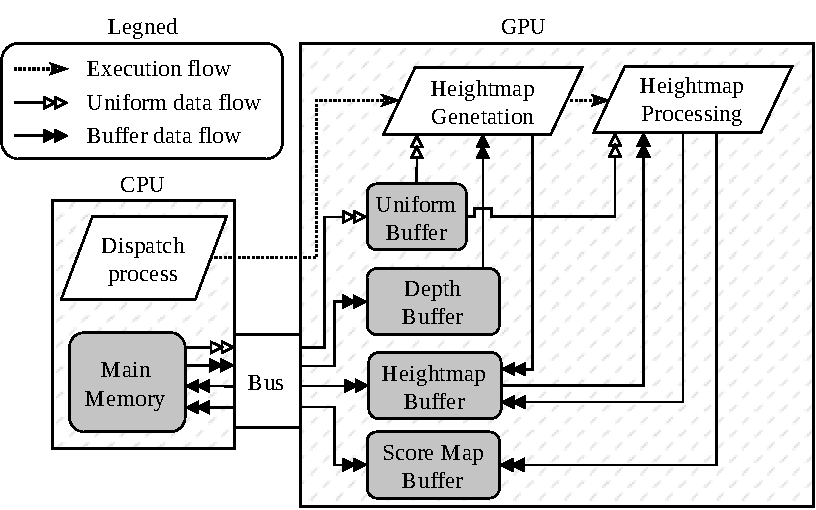
\includegraphics{Diagrams-ComputePipeline.drawio.pdf}
        \caption{Compute pipeline.}
        \label{fig:compute_pipe}
    \end{figure}

    \noindent
    As seen from figure \ref{fig:compute_pipe} the \ac{gpu} pipeline is relatively simple, being comprised of only two stages, the heightmap generation
    stage and the heightmap processing stage. The heightmap generation stage executes for each pixel on the depth image, constructing the heightmap as 
    described in chapter \ref{chap:mapping}.
    
    After the heightmap has been generated, the heightmap processing stage operates over the heightmap buffer. This stage has two tasks, to erase the
    old height data as the robot walks around, and to generate the score map, as described in section \ref{sec:scores}.
    
    \subsection{A note on \ac{gpu} architecture}
    A process on a \ac{gpu} operates fully in parallel and the \ac{gpu} is highly optimised for parallelisation, thus there is a very specific
    execution structure that a \ac{gpu} process abide by to perform at maximum efficiency, or to even function at all. This execution structure is
    as follows.
    
    When writing compute code a 3D size is specified, the localgroup size, \(\bm{N}_{l} = [X_l,Y_{l},Z_{l}]\), next when the \ac{cpu} dispatches
    a compute task, the workgroup count, is fed as parameter, \(\bm{n}_{w} = [x_{w},y_{w},z_{w}]\). The \ac{gpu} then initialises
    \(\bm{n}_w\) workgroups, and each workgroup initialises \(\bm{N}_l\) threads. These threads are grouped into warps, or waves, which, depending on the architectures processor count,
    can be either 32 or 64 threads. To ensure maximum efficiency it is important that \(\bm{N}_l\) is divisible by the warp size.
    Originally Nvidia \ac{gpu}s utilised a warp size of 32 and AMD 64, however with AMDs latest RDNA architecture, the warp size could be either 32 or 64.
    This system assumes a warp size of 32.
    
    For the heightmap generation stage \(\bm{N}_{l} = [32,32,0]\) for a total of 1024 threads per workgroup, or in other words, 32 warps per workgroup.
    As for the heightmap processing stage, \(\bm{N}_{l} = [32,32,32]\), meaning 32768 threads, or 1024 warps per workgroup.
    As such it is important that camera images, the heightmap and the score map are of a size divisible by 32.
    % A basic diagram of this execution scheme can be seen in figure \ref{fig:gpu_scheme}.
    % \begin{figure}[h]
    %     \centering
    %     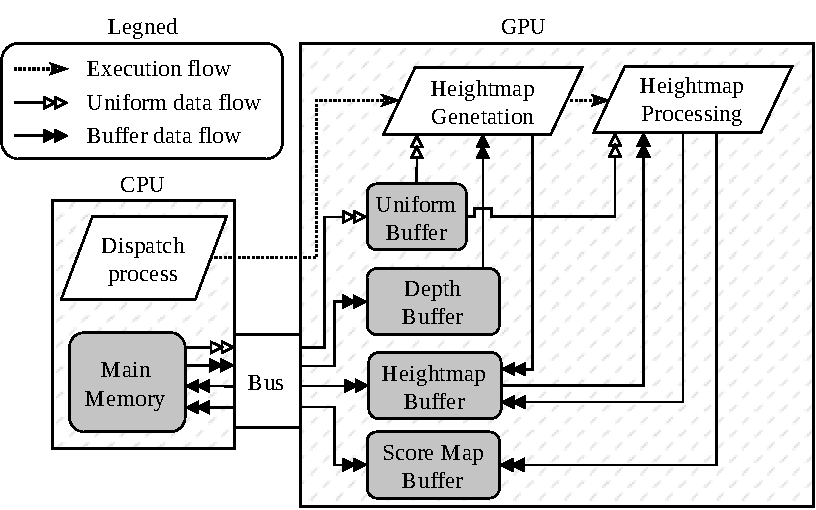
\includegraphics{Diagrams-ComputePipeline.drawio.pdf}
    %     \caption{GPU execution scheme.}
    %     \label{fig:gpu_scheme}
    % \end{figure}

    % \noindent
    While threads can directly communicate with each other within the same workgroup, direct communication across workgroups is
    impossible. If cross workgroup communication is desired, this must be performed using \ac{gpu} buffers, which are slower to access. Thus processes are
    designed to operate fully independently from each other. Of course, data transfer between the \ac{cpu} and the \ac{gpu} is orders of magnitudes
    slower than accessing local buffers, as such, all \ac{cpu}, \ac{gpu} is kept to a minimum.
    
    Finally it should be noted that while it is possible to vary \(\bm{s_w}\) with each execution cycle, \(\bm{S_l}\) is a constant specified at compile time,
    and as such the number of threads per workgroup cannot be altered during operation.

\bigskip
\hrule
\smallbreak
\hrule